\documentclass{article}
\usepackage{graphicx}
\graphicspath{ {./images/} }
\usepackage[export]{adjustbox}
\usepackage{amsmath}


\title{13. Polinomi. Gredzeni.}
\author{Gunārs Ābeltiņš}
\date{2022-05-20}

\begin{document}

\maketitle

\section*{1. Uzdevums}
\subsubsection*{Uzbūvējiet polinomu P(x), kas pieņem šādas vērtības: P(-3)=2; P(-1)=-2; P(0)=1; P(1)=-1; P(3)=1. Vienādojumu sistēmu atrisiniet ar WA. Vai atradīsiet, kā uzzīmēt iegūtā polinoma grafiku}

\begin{equation*}
    P(x) = a_4 x^4 + a_3 x^3 + a_2 x^2 + a_1 x + a_0
\end{equation*}

\begin{equation*}
    P(-3) = a_4 (-3)^4 + a_3 (-3)^3 + a_2 (-3)^2 + a_1 (-3) + a_0 = 2
\end{equation*}
\begin{equation*}
    P(-1) = a_4 (-1)^4 + a_3 (-1)^3 + a_2 (-1)^2 + a_1 (-1) + a_0 = -2
\end{equation*}
\begin{equation*}
    P(0) = a_4 (0)^4 + a_3 (0)^3 + a_2 (0)^2 + a_1 (0) + a_0 = 1
\end{equation*}
\begin{equation*}
    P(1) = a_4 (1)^4 + a_3 (1)^3 + a_2 (1)^2 + a_1 (1) + a_0 = -1
\end{equation*}
\begin{equation*}
    P(3) = a_4 (3)^4 + a_3 (3)^3 + a_2 (3)^2 + a_1 (3) + a_0 = 1
\end{equation*}

\begin{equation*}
    \begin{cases}
        81a_4 - 27a_3 + 9a_2 - 3a_1 + a_0 = 2 \\
        a_4 - a_3 + a_2 - a_1 + a_0 = -2      \\
        a_0 = 1                               \\
        a_4 + a_3 + a_2 + a_1 + a_0 = -1      \\
        81a_4 + 27a_3 + 9a_2 + 3a_1 + a_0 = 1
    \end{cases}
\end{equation*}

\begin{equation*}
    P(x) = \frac{23}{72} x^4 - \frac{1}{12} x^3 - \frac{203}{72} x^2 + \frac{7}{12} x + 1
\end{equation*}
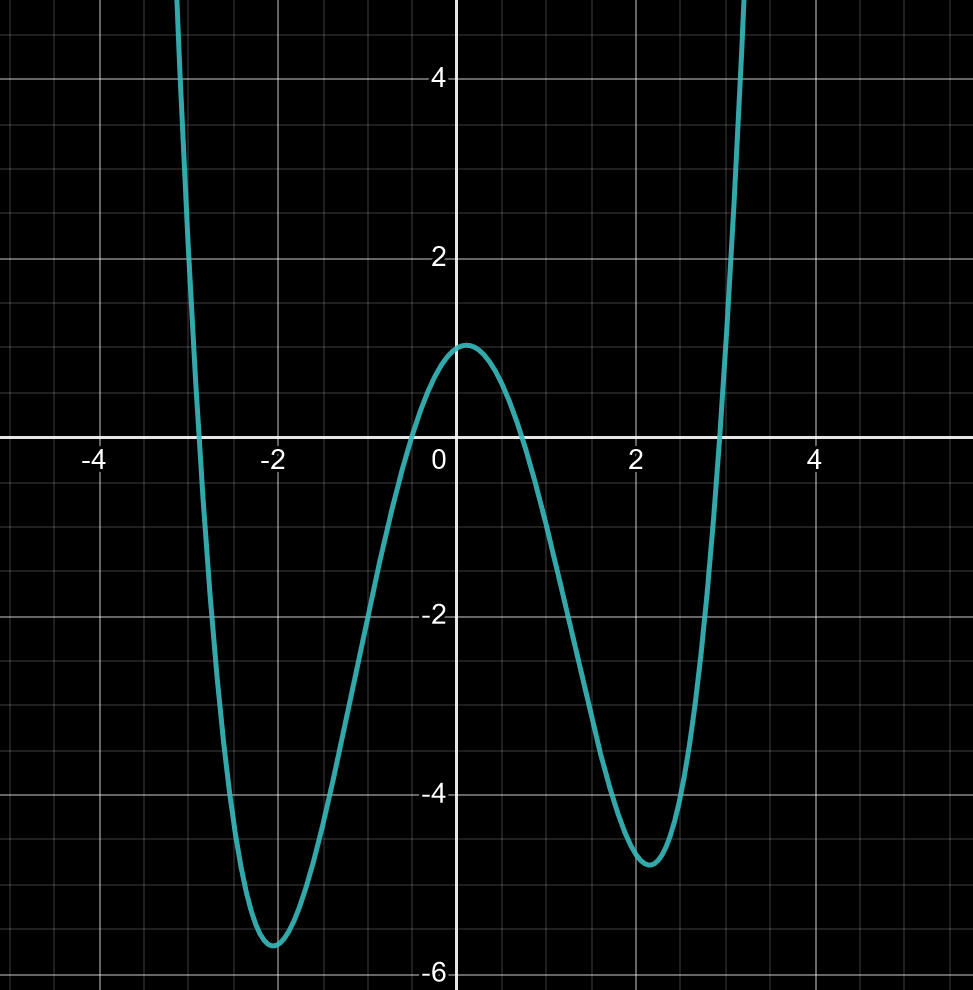
\includegraphics[width=0.9\textwidth, center]{1}

\section*{2. Uzdevums}
\subsubsection*{Izmantojot tikai gredzena aksiomas un jau iepriekš pierādītās teorēmas, pierādiet T6. Pamatojiet katru secinājumu soli.}

T6. Jebkurā gredzenā jebkuram a: $0*a=a*0=0$.
\\
Aplūkosim izteiksmes:
\begin{equation*}
    (a+0)*a ; a*(a+0)
\end{equation*}
3. gredzena aksioma:
\begin{equation*}
    a+0=a
\end{equation*}
Ņemot vērā 3. gredzena aksiomu, iegūstam:
\begin{equation*}
    (a+0)*a = a*a; a*(a+0) = a*a
\end{equation*}
7. gredzena aksioma:
\begin{equation*}
    a*(b+c)=(a*b)+(a*c);(b+c)*a=(b*a)+(c*a)
\end{equation*}
Ņemot vērā 7. gredzena aksiomu, iegūstam:
\begin{equation*}
    (a+0)*a = (a*a)+(0*a); a*(a+0) = (a*a)+(a*0)
\end{equation*}
Apvienojot iegūtās izteiksmes, iegūstam:
\begin{equation*}
    (a*a)+(0*a) = a*a; (a*a)+(a*0) = a*a
\end{equation*}
Atņemot no abām pusēm $a*a$, iegūstam:
\begin{equation*}
    0*a = 0; a*0 = 0
\end{equation*}
Q.E.D.

\section*{3. Uzdevums}
\subsubsection*{Izmantojot tikai gredzena aksiomas un jau iepriekš pierādītās teorēmas, pierādiet  T6'. Pamatojiet katru secinājumu soli.}

T6'. Jebkurā gredzenā distributīvie likumi
izpildās arī atņemšanai:
\begin{equation*}
    a*(b-c)=a*b-a*c; (b-c)*a=b*a-c*a
\end{equation*}
Ieviesīsim:
\begin{equation*}
    b-c=x; x+c=b
\end{equation*}
Aplūkosim izteiksmes:
\begin{equation*}
    a*(x+c)=a*b; (x+c)*a=b*a
\end{equation*}
Ņemot vērā 7. gredzena aksiomu, iegūstam:
\begin{equation*}
    a*x+a*c=a*b; x*a+c*a=b*a
\end{equation*}
Atņemama no abām pusēm $a*c$ un $c*a$ respektīvi, iegūstam:
\begin{equation*}
    a*x=a*b-a*c; x*a=b*a-c*a
\end{equation*}
Ievietojot $x=b-c$, iegūstam:
\begin{equation*}
    a*(b-c)=a*b-a*c; (b-c)*a=b*a-c*a
\end{equation*}
Q.E.D.

\end{document}